%\setcounter{section}{0}
\section{Premier développement sur Contiki}
Pour mieux appréhender la variété de l'environnement et des outils la première tâche qui m'a été confiée n'était pas au cœur de ses systèmes. J'ai tout d'abord lu l'article \citep{acostapadilla} pour me familiariser avec cet environnement. 

Les nœuds \emph{m3} étant uniquement capable d'exécuter du code déjà compilé il a fallu que je mette en place un environnement dit de \emph{Cross-compilation}, ou compilation croisée, qui consiste à produire un code binaire exécutable par une machine ayant une architecture différente de celle servant au développement.

Pour développer un nouveau module pour \emph{Contiki} il suffit d'en récupérer les sources\footnote{https://github.com/iot-lab/contiki}, de se placer dans le répertoire contenant les sources d'un module et de le compiler en précisant l'architecture cible, iotlab-m3.

\lstset{language=bash, captionpos=b, caption=Résumé des étapes de compilation}
\begin{lstlisting}[frame=single]
git clone https://github.com/iot-lab/contiki
cd contiki/example/hello-world
make TARGET=iotlab-m3
\end{lstlisting}

Cette compilation produira un firmware contenant \emph{Contiki}, le module courant ainsi que tout autre module marqué en dépendance. Ce firmware pourra directement être flashé sur un nœud \emph{m3}.

\section{Compression des modèles}

Pour pouvoir s'adapter et selon le principe du \emph{model@runtime} chaque nœud d'un réseau IoT doit comparer le nouveau modèle du réseau avec le courant et en déduire s'il doit se modifier. Il est donc nécessaire que le nouveau modèle soit échangé entre tous les nœuds. Dans un soucis de temps de développement et puisque cela n'impacte pas l'idée de \emph{model@runtime} l'implémentation de \emph{kevoree-c} ne compresse pas les modèles avant de les transmettre aux pairs voisins.

\subsection{État de l'art}

Puisque aucun algorithme de compression de données n'est fourni avec \emph{Contiki} j'ai d'abord commencé par en chercher implémentés en \emph{C}, recommandés pour les systèmes embarqués et disponibles en sources libres dans des licences permettant leurs réutilisations.

L'objectif étant d'avoir le meilleur taux de compression tout en restant le moins demandeur de ressources matérielles, en particulier en mémoire RAM.

Les implémentations retenues et étudiées sont \emph{Huffman}, \emph{fastlz}\footnote{http://fastlz.org/} et \emph{lzf} \footnote{http://oldhome.schmorp.de/marc/liblzf.html}.

Les résultats ont été obtenus en utilisant l'outil \emph{Massif}\footnote{http://valgrind.org/docs/manual/ms-manual.html} de la suite d'outils Valgrind. \emph{Massif} permet de mesurer l'utilisation de différentes zones mémoire lors de l'exécution d'un programme. Par défaut seul l'utilisation du tas est mesuré mais la pile peut également l'être après configuration. Les fichiers de données produits sont binaires mais peuvent être visualisés à l'aide de l'outil \emph{msprint} fourni avec \emph{Massif}.

Les mesures étant faites sur un ordinateur classique d'architecture 64bit et non sur l'environnement de production la compilation a été réalisée en 32bit pour réduire la taille des adresses de pointeur manipulées et ainsi avoir des résultats plus fiables. Tous les algorithmes ont été utilisés en compression et en décompression sur plusieurs modèles différents représentatifs de ceux utilisés lors des expériences.

Les scripts utilisés pour automatiser les mesures et produire les résultats suivants sont disponibles sur Github\footnote{https://github.com/AlexandreRio/embedded-compression-benchmark}.

\subsection{Résultats mesurés}

Le taux de compression $\frac{taille~finale}{taille~initiale}$ moyens de chaque algorithme est mesuré sur un ensemble de fichier 14 fichiers représentant 7 modèles différents. Chaque modèle est représenté par un fichier facilement lisible par l'Homme et par une représentation minimaliste, sans caractère de mise en forme superflu.
\[
\begin{array}{lc}
Algorithme & Taux~de~compression \\
LZF & 0.174 \\
Huffman & 0.604 \\
Fastlz-1 & 0.179 \\
Fastlz-2 & 0.171 \\
Table~association & 0.641
\end{array}
\]

L'annexe \ref{comp-tabde} détaille les tailles avant et après compression pour l'ensemble de ces fichiers.

\begin{figure}[ht!]
\centering
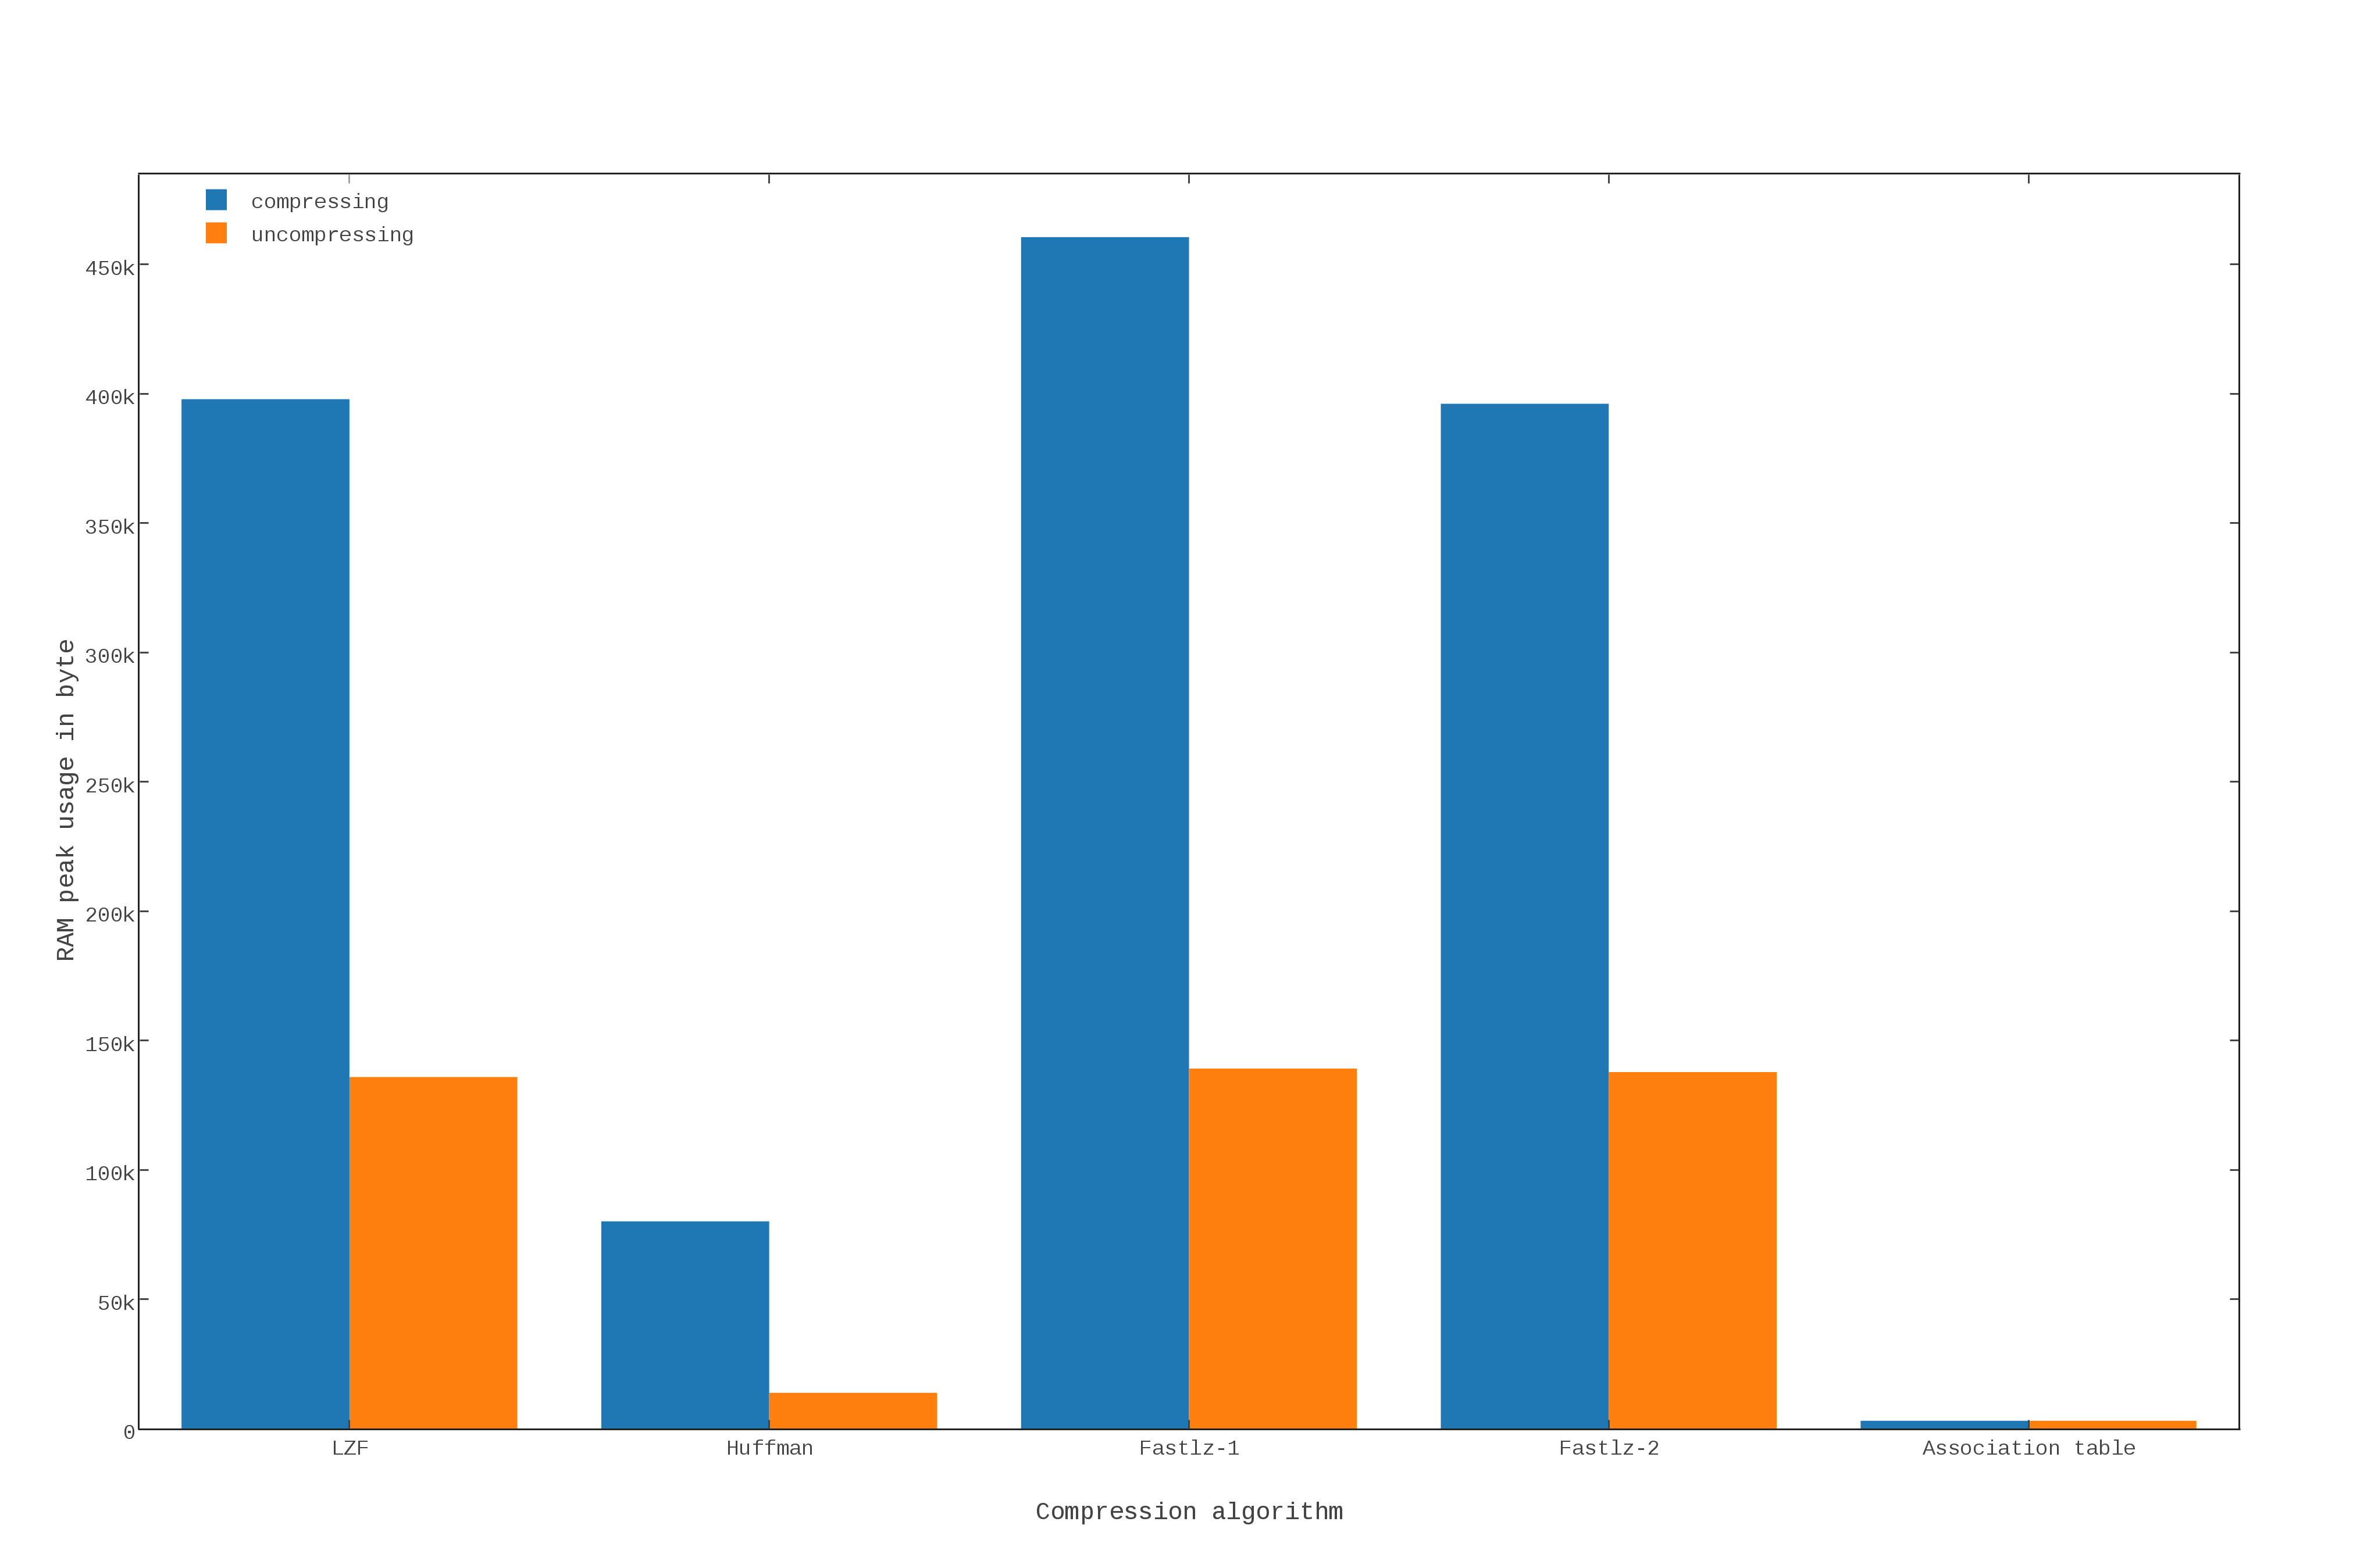
\includegraphics[scale=0.4]{images/comp-memory.png}
\caption{Pic moyen d'utilisation de la RAM en octet en fonction de l'algorithme de compression.}
\end{figure}

En réduisant la taille des buffers la taux de compression chute

\subsection{Table d'association}

Vue qu'aucune implémentation existante ne peut fonctionner sur \emph{Contiki} j'ai développé un programme de compression.

La structure générale et les mots-clés du fichier à compresser étant connus à l'avance la méthode la plus simple de compression est de réaliser une table d'association entre les mots les plus fréquemment utilisés et de les substituer par un code plus court.

Cette approche oblige tous les nœuds à connaître la table d'association utilisée pour compresser lors de la décompression. Cette table étant constante lors de la vie du programme elle peut être stockée en ROM, ce qui est important dans notre cas.

Pour obtenir cette table d'association j'ai réalisé un programme \emph{Java}, disponible sur Github\footnote{https://github.com/AlexandreRio/Contiki-compression-tools}, qui se base sur un ensemble de modèle. Le programme peut être paramétré pour produire une table plus au moins grosse, au détriment du taux de compression moyen.

Les premiers tests sur \emph{Contiki} ont d'abord consisté à simplement compressé une   chaine de caractères constante au programme, puis un fichier local au nœud et pour finir un fichier local au nœud envoyé à un second nœud qui le décompresse après réception. Le résultat attendu étant que le fichier obtenu après compression, transmission et décompression soit identique ou au moins sémantiquement identique.

Les expériences ont été réalisées sur le testbed FIT IoT-lab de Rocquencourt qui a l'avantage de ne compter que 24 nœuds M3 (voir annexe \ref{iot-lab}), ce qui est largement suffisant dans le cadre de cette expérience et permet d'être sur d'avoir des nœuds disponibles et de pouvoir les réserver pour plusieurs heures sans gêner d'autres expériences.

La transmission de données, ici de modèles, est particulière sur un réseau mesh et dans le cas de \emph{Kevoree}. Pour le \emph{model@runtime} la transmission de données est utilisée pour transmettre le nouveau modèle depuis $1$ nœud à $n-1$ nœuds, cette transmission a été appelée dissémination. Dans le cadre de mes expériences de test de compression avant transmission j'ai déployer plusieurs nœuds \emph{border router} possédant la nouvelle version du modèle et seulement $1$ possédant l'ancienne version. De cette manière et en prenant en compte comment l'algorithme de dissémination est implémentée le nœud possédant l'ancienne version pourra recevoir la nouvelle, découpées en morceaux, de tous les nœuds proches de lui et ainsi le recevoir plus vite et donc réduire le temps des expériences et par extension mon temps de développement.

Après avoir résolu les différents bugs liés à l'environnement, tel que le système de fichier, le code du programme de compression a déplacer afin de produire un module indépendant dans \emph{Contiki}. De ce fait n'importe quel autre module ou programme basé sur \emph{Contiki} peut utiliser cette fonction pour compresser ou décompresser des fichiers.

% vérifier les liens
Les sources de la version de compression seule \footnote{https://github.com/AlexandreRio/contiki/tree/usingOldKevoree/examples/compress} et de la compression et transmission \footnote{https://github.com/AlexandreRio/contiki/tree/usingOldKevoree/examples/compress-disseminate} sont disponibles sur Github.

\section{Parser spécifique}

\subsection{Tentatives de portage}

trop de limite,
\section{Compilation}

Le gros du stage pour le moment

\subsection{L'intérêt de générer du code}

\subsection{Un vrai compilateur et pas juste une transcription de modèle}